\section{Введение}
Магнитные свойства важны в различных областях, включая материаловедение и химию. Понимание поведения магнитных моделей на ансамблях конформаций молекул имеет решающее значение как для фундаментальных исследований, так и для практических приложений. В этом исследовании мы стремимся исследовать свойства магнитных моделей ансамблей конформаций молекул.

Чтобы сгенерировать ансамбли конформаций, мы будем использовать широко используемый метод, называемый самоизбегающим случайным блужданием (SAW). Этот метод генерирует конформации, которые точно отражают поведение молекул в растворе. Для изучения магнитных свойств молекул воспользуемся моделью Изинга \cite{ising}. Модель Изинга — это математическая модель, описывающая поведение магнитных систем, включая взаимодействия между магнитными моментами и внешним магнитным полем.

\begin{figure}[h]
	\centering
    \begin{subfigure}{0.45\textwidth}
        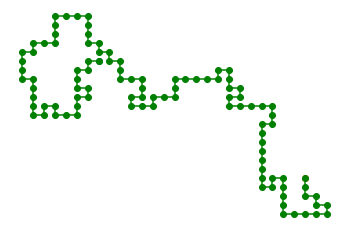
\includegraphics[width=\textwidth]{../images/loose_conf.png}
        \caption{глобула}
    \end{subfigure}
    \begin{subfigure}{0.45\textwidth}
	    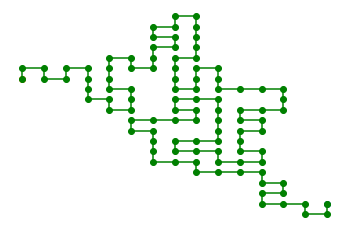
\includegraphics[width=\textwidth]{../images/dense_conf.png}
        \caption{клубок}
    \end{subfigure} 
	\caption{Примеры конформаций}
    \label{fig::globule_coil_example}
\end{figure}

Нас особенно интересуют эти модели из-за их уже известных свойств. Точное решение для модели Изинга \cite{ising_solutions} показывает, что на одномерной сетке модель Изинга не имеет магнитного фазового перехода, одномерная модель не становится магнитной ни при каких температурах, кроме абсолютного нуля. Но в модели есть фазовый переход на двумерной сетке. Двумерная сетка становится магнитной при низких температурах. И конформации тоже имеют фазовый переход. Два состояния называются глобулой и клубком и соответствуют низким и высоким температурам, пример конформаций представлен на Рис. \ref{fig::globule_coil_example}. Структурно состояния конформации, которые в основном проявляются в глобулах и клубках, подобны одномерным и двумерным сеткам соответственно. Учитывая эти факты, можно предположить, что глобулярные конформации имеют магнитный фазовый переход, а клубки — нет.

Основная цель этой работы - определить существование магнитного фазового перехода модели Изинга на конформациях замороженной глобулы и клубка. Если фазовый переход существует, найдите точную температуру перехода и сравните ее с температурой геометрического перехода для конформаций. В целом, этот проект направлен на углубление нашего понимания свойств магнитных моделей ансамблей конформаций молекул. Знания, полученные в ходе этого проекта, могут найти применение в различных областях, например, при разработке новых материалов с желаемыми магнитными свойствами.